\documentclass{beamer}
\usepackage{tikz}
\usetikzlibrary{positioning}
%
% Choose how your presentation looks.
%
% For more themes, color themes and font themes, see:
% http://deic.uab.es/~iblanes/beamer_gallery/index_by_theme.html
%
\mode<presentation>
{
  \usetheme{Madrid}      % or try Darmstadt, Madrid, Warsaw, ...
  \usecolortheme{default} % or try albatross, beaver, crane, ...
  \usefonttheme{default}  % or try serif, structurebold, ...
  
  \setbeamertemplate{navigation symbols}{}
  \setbeamertemplate{caption}[numbered]
} 

\usepackage[english]{babel}
\usepackage[utf8x]{inputenc}

\title[Neural Networks]{Introduction to Neural Networks}
\author{Gautom Das, Liam DeVoe, \& Natnael Kelkay}
\institute{Montgomery Blair High School}
\date{\today}

\begin{document}

\begin{frame}
  \titlepage
\end{frame}

% Uncomment these lines for an automatically generated outline.
%\begin{frame}{Outline}
%  \tableofcontents
%\end{frame}

\section{Introduction}

\begin{frame}{Objectives}

\begin{enumerate}
	\item Understand how neural networks came about
	\newline
	\item Neural networks are not special
\end{enumerate}
\end{frame}

\begin{frame}{Background}
Let's travel back to 

\end{frame}


\begin{frame}{Introduction}

\begin{figure}
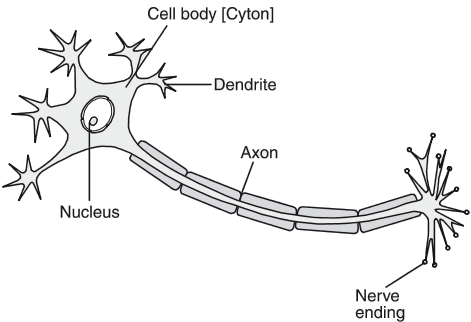
\includegraphics[width=0.65\textwidth]{12img}
\end{figure}


\vskip -0.3cm

\begin{block}{Theory}
Let's start with a single neuron from the brain. Dendrites feed information into it, then there is the body of the neuron that performs some 'biology' operation on the inputs then outputs this information with its axons.
\end{block}

\end{frame}

\begin{frame}{Single Neuron Construction}
With this is in mind, let's try to model a single neuron mathematically:
\begin{center}
	\begin{tikzpicture}
	\draw (0,0) circle (1cm);
	\draw [->] (-4,1.75) -- (-1,0.6);
	\node[draw] at (-4.5,1.8) {$x_1$};
	
	\draw [->] (-4, 0.55) -- (-1.1,0.2);
	\node[draw] at (-4.5, 0.55) {$x_2$};
	
	\draw [fill] (-4.5,-0.15) circle [radius=0.075];
	\draw [fill] (-4.5,-0.55) circle [radius=0.075];
	\draw [fill] (-4.5,-0.95) circle [radius=0.075];
	
	\draw [->] (-4,-1.75) -- (-1,-0.6);
	\node[draw] at (-4.5,-1.8) {$x_i$};
	
	\draw [->] (1.1,0) -- (4.0,0);
	\node[draw] at (4.6,0) {$O_n$};
	
	\node[text width=3cm, align=center,font=\Large] at (0,0) 
    {\textbf{$\Sigma $}};
    
    
	\end{tikzpicture}
\end{center}
Our input denoted by $x_i$ have our inputs and then flow into the 'nucleus' of the neuron. There, a function is performed on all of the inputs and that information is then passed to another neuron or neurons.

\end{frame}

\begin{frame}{Single Neuron Construction}

\begin{center}
	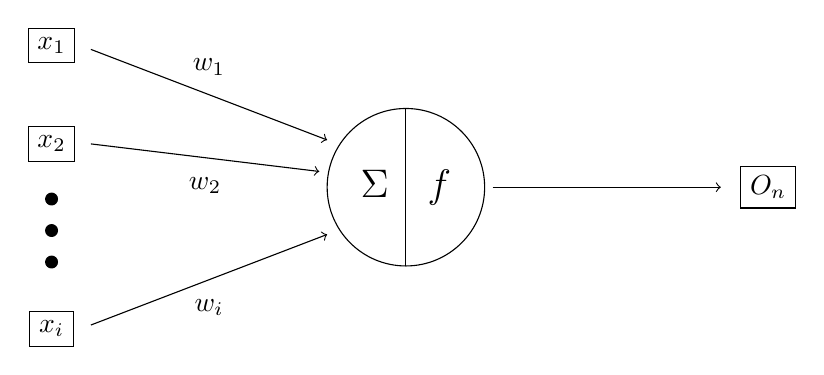
\begin{tikzpicture}
	\draw (0,0) circle (1cm);
	\draw [->] (-4,1.75) -- node[label= above:$w_1$] {} (-1,0.6);
	\node[draw] at (-4.5,1.8) {$x_1$};
	
	\draw [->] (-4, 0.55) -- node[label= below:$w_2$]  {} (-1.1,0.2);
	\node[draw] at (-4.5, 0.55) {$x_2$};
	
	\draw [fill] (-4.5,-0.15) circle [radius=0.075];
	\draw [fill] (-4.5,-0.55) circle [radius=0.075];
	\draw [fill] (-4.5,-0.95) circle [radius=0.075];
	
	\draw (0,1) -- (0,-1);
	
	\draw [->] (-4,-1.75) -- node[label= below:$w_i$]  {} (-1,-0.6);
	\node[draw] at (-4.5,-1.8) {$x_i$};
	
	\draw [->] (1.1,0) -- (4.0,0);
	\node[draw] at (4.6,0) {$O_n$};
	
	\node[text width=3cm, align=center,font=\Large] at (0,0) 
    {\textbf{$\Sigma \:  \:\:  f$}};
    
    
	\end{tikzpicture}
	
\end{center}

\begin{block}{Neuron Formula}
For a given neuron we can get the following formula:
$$
O_n = \sigma \Big(\sum_{i=1}^{n}{x_iw_i} + b \Big)
$$
\end{block}


\end{frame}

\begin{frame}{Full Neural Network}

\tikzset{%
  every neuron/.style={
    circle,
    draw,
    minimum size=1cm
  },
  neuron missing/.style={
    draw=none, 
    scale=4,
    text height=0.333cm,
    execute at begin node=\color{black}$\vdots$
  },
}

\begin{figure}[htbp]
	\centering
\hspace*{-4.5cm}
\vspace*{-2.5cm}
\begin{tikzpicture}[x=1.6cm, y=1.5cm, >=stealth, transform canvas={scale=0.75}]

\foreach \m/\l [count=\y] in {1,2,missing,3}
  \node [every neuron/.try, neuron \m/.try] (input-\m) at (0,2.5-\y) {};

\foreach \m [count=\y] in {1, 2,missing,3}
  \node [every neuron/.try, neuron \m/.try ] (hidden-\m) at (2,3.2-\y*1.25) {};

\foreach \m [count=\y] in {1,missing,2}
  \node [every neuron/.try, neuron \m/.try ] (output-\m) at (4,2.0-\y) {};

\foreach \l [count=\i] in {1,2,n}
  \draw [<-] (input-\i) -- ++(-1,0)
    node [above, midway] {$I_\l$};

\foreach \l [count=\i] in {1,2,n}
  \node [above] at (hidden-\i.north) {$H_\l$};

\foreach \l [count=\i] in {1,n}
  \draw [->] (output-\i) -- ++(1,0)
    node [above, midway] {$O_\l$};

\foreach \i in {1,...,3}
  \foreach \j in {1,...,3}
    \draw [->] (input-\i) -- (hidden-\j);

\foreach \i in {1,...,3}
  \foreach \j in {1,...,2}
    \draw [->] (hidden-\i) -- (output-\j);

\foreach \l [count=\x from 0] in {Input, Hidden, Ouput}
  \node [align=center, above] at (\x*2,2.7) {\l \\ layer};

\end{tikzpicture}

\end{figure}

\end{frame}

\subsection{Mathematics}

\begin{frame}{Readable Mathematics}

Let $X_1, X_2, \ldots, X_n$ be a sequence of independent and identically distributed random variables with $\text{E}[X_i] = \mu$ and $\text{Var}[X_i] = \sigma^2 < \infty$, and let
$$S_n = \frac{X_1 + X_2 + \cdots + X_n}{n}
      = \frac{1}{n}\sum_{i}^{n} X_i$$
denote their mean. Then as $n$ approaches infinity, the random variables $\sqrt{n}(S_n - \mu)$ converge in distribution to a normal $\mathcal{N}(0, \sigma^2)$.

\end{frame}

\end{document}
